\documentclass[12pt]{article}
\usepackage{titletoc}

\usepackage{sectsty}
\sectionfont{\fontsize{20}{18}\selectfont}
\subsectionfont{\fontsize{18}{18}\selectfont}
\subsubsectionfont{\fontsize{16}{18}\selectfont}

\usepackage{mathptmx}
\renewcommand*\rmdefault{mathptmx}




\usepackage{ucs}
\usepackage[utf8x]{inputenc} % Включаем поддержку UTF8
\usepackage[russian]{babel}  % Включаем пакет для поддержки русского языка

\usepackage[left=2cm, 		% Поле левое : 200 мм
			right=2cm, 		% Поле правое : 200 мм
			top=1cm,		% Поле верхнее: 100 мм
			bottom=2cm,		% Поле нижнее : 200 мм
			bindingoffset=0cm]{geometry}
			
\usepackage[pdftex]{graphicx, color}
\usepackage{color}
\usepackage{wrapfig}
\usepackage{float}
\usepackage{tikz}
 \usepackage{url}			% использование URL в библиографии
\usepackage{listings}		% использование листингов кода
\usepackage[nooneline]{caption} 
\captionsetup[table]{justification=raggedleft} 
\captionsetup[figure]{justification=centering,labelsep=endash}
\usepackage{array}

\usepackage{caption}
\usepackage{graphicx}


\renewcommand{\baselinestretch}{1.5}

% вставка листингов с кодом 
\lstset{inputencoding=utf8x, 		
		extendedchars=false, 
		keepspaces=true,
		language=c}

\renewcommand{\lstlistingname}{Листинг}
\usepackage[indentfirst,compact,topmarks,calcwidth,pagestyles]{titlesec}

%\usepackage{amsmath}
%\usepackage{mathtools}
\def\checkmark{\tikz\fill[scale=0.4](0,.35) -- (.25,0) -- (1,.7) -- (.25,.15) -- cycle;} 
\setcounter{tocdepth}{4} 	% chapter, section, subsection, subsubsection и paragraph
\setcounter{secnumdepth}{4}

\parindent=1,25cm				% красная строка = 1 см
\usepackage{enumitem}
\setlist[enumerate,1]{leftmargin=2.25cm}
\setlist[itemize]{leftmargin=2.25cm}
\graphicspath{{pics/}}
\DeclareGraphicsExtensions{{.jpg}}

\begin{document}
\fontsize{14}{16pt}\selectfont


	\begin{titlepage}
	
	\end{titlepage}

	
	\tableofcontents %Содержание
	\newpage
	
	
%====================================================================================
%Введение
%====================================================================================
	\part*{\centering Введение}
	\addcontentsline{toc}{part}{Введение}
Развитие информационных технологий ведет к формированию новых возможностей в применении вычислительных мощностей компьютера для решения разного  рода задач. Повсеместно распространяются новые технологии, такие как: умный дом, интернет вещей, техническое зрение и мное другое. И все эти новые технологии становятся неотъемлемой частью нашей жизни и иногда кажется неразумный, когда простейшие операции выполняются людьми, а могли бы выполнятся компьютерами или роботами. В связи с чем, у пытливых умов, возникают разного рода идеи по рационализации деятельности человека.
\\  \indent Одним из бурно развивающихся направлений является техническое зрение. Сейчас можно сказать, что большая часть фундаментальных основ для данной технологии уже заложено и появляющиеся новые языки программирования и специализированные библиотеки делаю это занятием весьма доступными для человека нового в данной области. 
\\  \indent  Изучая в университете курс имитационного моделирования я проникся идеей имитации поведения реального объекта в виртуальном мире. Многообразие существующих методов моделирования позволяет создавать модели практически любого объекта. Буть то молекулярная модель невидимого, без дополнительного оборудования,  для для человеческого глаза объекта или вполне заметная модель крупного завода. Так мне досталась одна такая задача из объектов окружаемой нас действительности,  а именно одна из станций московского метро. Во время создания модели станции передомной стояла задача моделирования пассажиропотоков на станции, как несложно догадаться, задачу подсчета количества пассажиров выполнялась в виде наблюдения и фиксирования их количества. Занятие весьма и весьма монотонное и малоинтересное. 
\\  \indent В связи с чем возникла идея попробовать автоматизировать эту задачу. Немного поразмыслив пришла идея анализа видео с камер видеонаблюдения, которые установлены практически в любом месте скопления людей. 


	\hspace{\parindent}

%====================================================================================	
	\newpage
	\section{Предпроектное исследование}
		\subsection{Основы компьютерного зрения}

Как научная дисциплина, компьютерное зрение относится к теории и технологии создания искусственных систем, которые получают информацию из изображений. Видеоданные могут быть представлены множеством форм, таких как видеопоследовательность, изображения с различных камер или трехмерными данными, например с устройства Kinect или медицинского сканера.
Как технологическая дисциплина, компьютерное зрение стремится применить теории и модели компьютерного зрения к созданию систем компьютерного зрения. Примерами применения таких систем могут быть:
\begin{itemize}
\item Системы управления процессами (промышленные роботы, автономные транспортные средства)
\item Системы видеонаблюдения
\item Системы организации информации (например, для индексации баз данных изображений)
\item Системы моделирования объектов или окружающей среды (анализ медицинских изображений, топографическое моделирование)
\item Системы взаимодействия (например, устройства ввода для системы человеко-машинного взаимодействия)
\item Системы дополненной реальности
\item Вычислительная фотография, например для мобильных устройств с камерами
\end{itemize}

Компьютерное зрение также может быть описано как дополнение (но не обязательно противоположность) биологическому зрению. В биологии изучается зрительное восприятие человека и различных животных, в результате чего создаются модели работы таких систем в терминах физиологических процессов. Компьютерное зрение, с другой стороны, изучает и описывает системы компьютерного зрения, которые выполнены аппаратно или программно. Междисциплинарный обмен между биологическим и компьютерным зрением оказался весьма продуктивным для обеих научных областей.
Подразделы компьютерного зрения включают воспроизведение действий, обнаружение событий, слежение, распознавание образов, восстановление изображений и некоторые другие.[1]
\\  \indent Реализация систем компьютерного зрения сильно зависит от области их применения, аппаратной платформы и требований по производительности. Некоторые системы являются автономными и решают специфические проблемы детектирования и измерения, тогда как другие системы составляют под-системы более крупных систем, которые уже могут содержать подсистемы контроля механических манипуляторов (роботы), информационные базы данных (поиск похожих изображений), интерфейсы человек-машина и (компьютерные игры) т.д. Однако, существуют функции, типичные для многих систем компьютерного зрения.[2]
\\  \indent  Получение изображений: цифровые изображения получаются от одного или нескольких датчиков изображения, и которые помимо различных типов светочувствительных камер включают датчики расстояния, радары, ультразвуковые камеры и т. д. В зависимости от типа датчика, получающиеся данные могут быть обычным 2D изображением, 3D изображением или последовательностью изображений. Значения пикселей обычно соответствуют интенсивности света в одной или нескольких спектральных полосах (цветные или изображения в оттенках серого), но могут быть связаны с различными физическими измерениями, такими как глубина, поглощение или отражение звуковых или электромагнитных волн, или ядерным магнитным резонансом.[3]
\\  \indent  Предварительная обработка: перед тем, как методы компьютерного зрения могут быть применены к видеоданным с тем, чтобы извлечь определённую долю информации, необходимо обработать видеоданные, с тем чтобы они удовлетворяли некоторым условиям, в зависимости от используемого метода. Примерами являются:

\begin{itemize}
\item Повторная выборка с тем, чтобы убедиться, что координатная система изображения верна
\item Удаление шума с тем, чтобы удалить искажения, вносимые датчиком
\item Улучшение контрастности, для того, чтобы нужная информация могла быть обнаружена
\item Масштабирование для лучшего различения структур на изображении
\end{itemize}

  Выделение деталей: детали изображения различного уровня сложности выделяются из видеоданных. Типичными примерами таких деталей являются:
\begin{itemize}
\item Линии, границы и кромки
\item Локализованные точки интереса, такие как углы, капли или точки: более сложные детали могут относиться к структуре, форме или движению.
\end{itemize}
Детектирование/Сегментация: на определённом этапе обработки принимается решение о том, какие точки или участки изображения являются важными для дальнейшей обработки. Примерами являются:
\begin{itemize}
\item Выделение определённого набора интересующих точек
\item Сегментация одного или нескольких участков изображения, которые содержат характерный объект
\end{itemize}

 Высокоуровневая обработка: на этом шаге входные данные обычно представляют небольшой набор данных, например набор точек или участок изображения, в котором предположительно находится определённый объект. Примерами являются:
\begin{itemize}
\item Проверка того, что данные удовлетворяют условиям, зависящим от метода и применения
\item Оценка характерных параметров, таких как положение или размер объекта
\item Классификация обнаруженного объекта по различным категориям
\end{itemize}	
	\subsection {Основные положения библиотеки компьютерного зрения OpenCV }
OpenCV (англ. Open Source Computer Vision Library, библиотека компьютерного зрения с открытым исходным кодом) — библиотека алгоритмов компьютерного зрения, обработки изображений и численных алгоритмов общего назначения с открытым кодом. Реализована на C/C++, также разрабатывается для Python, Java, Ruby, Matlab, Lua и других языков. Может свободно использоваться в академических и коммерческих целях — распространяется в условиях лицензии BSD.

Применение:

\begin{itemize}
  \item Для утверждения общего стандартного интерфейса компьютерного зрения для приложений в этой области. Для способствования росту числа таких приложений и создания новых моделей использования PC
  \item Сделать платформы Intel привлекательными для разработчиков таких приложений за счёт дополнительного ускорения OpenCV с помощью Intel® Performance Libraries (Сейчас включают IPP (низкоуровневые библиотеки для обработки сигналов, изображений, а также медиа-кодеки) и MKL (специальная версия LAPACK и FFTPack)). OpenCV способна автоматически обнаруживать присутствие IPP и MKL и использовать их для ускорения обработки.
\end{itemize}

В версии 2.2 библиотека была реорганизована. Вместо универсальных модулей cxcore, cvaux, highGUI и других было создано несколько компактных модулей с более узкой специализацией.


 	\subsection{Поколения систем сбора статистики}
			\hspace{\parindent}

Еще до того как я определился с методом решения задачи подсчета пассажиров я попытался проанализировать существующие методики. И так поискав материалы из разного рода источников я сформировал вот такую таблицу. 

\begin{figure}[h!]
  \centering
    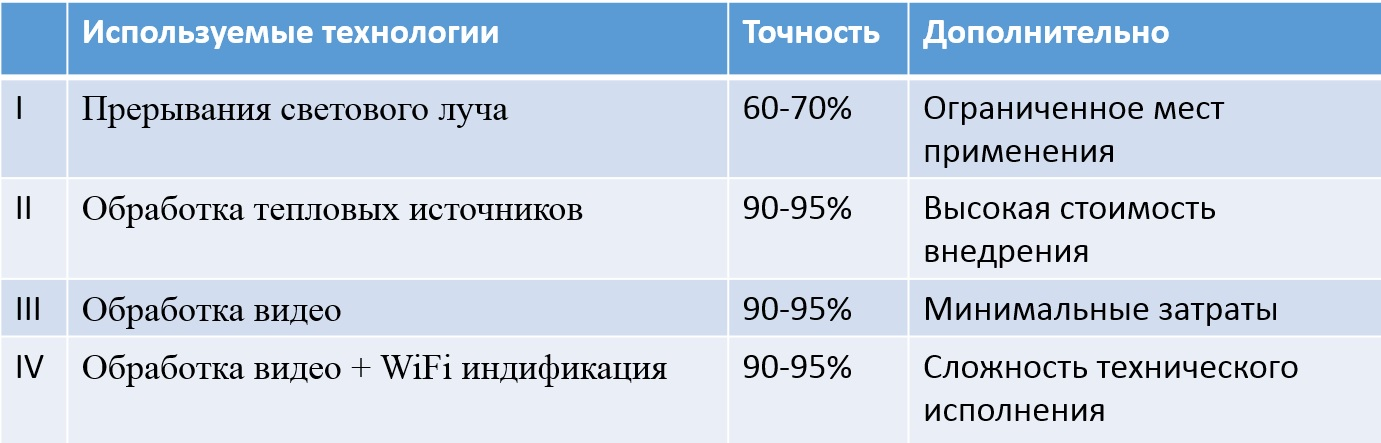
\includegraphics[width=0.8\textwidth]{pic/generation.jpg}
\end{figure}

На первых парах решения данной задачи активно использовались существующие методики по прерыванию светового луча. Так например в московском метро, но для цели предотвращения входа без билеты. По такому же принципу подсчитывали количество пассажиров.
\begin{figure}[h!]
  \centering
    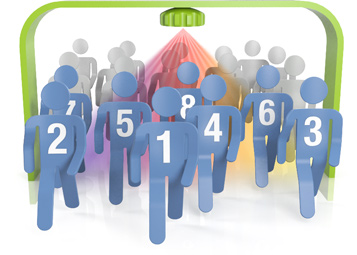
\includegraphics[width=0.3\textwidth]{pic/schem.jpg}
  \caption{Прерывания светового луча}
\end{figure}
 Другим направлением является обработка тепловых источников, а именно датчики срабатывающее на приближение объекта с определенной температурой, а в дальнейшем и камеры способные анализировать тепловые источники. Этот вариант самый подходящий для нас, но чрезмерно дорогостоящий.

\begin{figure}[h!]
  \centering
    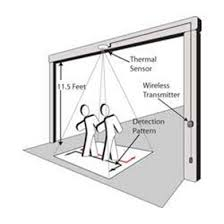
\includegraphics[width=0.3\textwidth]{pic/termal_counting.jpg}
  \caption{Обработка тепловых источников}
\end{figure}

 3-й подход это анализ видео с простые камер видеонаблюдения. Среди всех перечисленных эта технология имеет наименьшую стоимость и может применяться везде, где установлены системы видео наблюдения. 

\begin{figure}[h!]
  \centering
    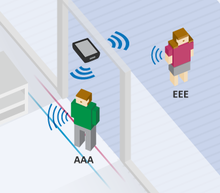
\includegraphics[width=0.3\textwidth]{pic/Wi-Fi_Tracking.png}
  \caption{Обработка видео + WiFi индификация}
\end{figure}

А вершиной развития этой идеи является сочетание анализа виде + индификация объектов по используемым mac адресам устройств 

		\subsection {Основные подходы в анализе видео}
			\hspace{\parindent}
До начала работы над проектом мной были изучены несколько популярных методов обработки видео реализованных  в OpenCV. 

\begin{itemize}
\item Непрерывная адаптация среднего сдвига (Camshift)
\item Оптический поток (Optical Flow)
\item Вычитание фона (Background Subtraction)
\item Машинное обучение (Machine Learning)
\item Обнаружение объекта  (Object Detection)
\end {itemize}

После анализа всем методов было принято решение использовать алгоритм вычитания фона.

\newpage

\section{Техническое задание}
	\subsection{Введение }	
Во время выполнения курсового проекта по теме "Моделирование транспортного узла станции метро Третьяковская"	 я столкнулся с задачей подсчета количества пассажиров выходящих из вагона метро. Подсчет количества пассажиров занимает много времени и тяжелого малоинтеллектуального труда. В связи с этим возникла идея автоматизировать подсчеты.  
	\subsection{Общие сведения }
	
	Основание для разработки: задание на курсовой проект.
	
	Заказчик: Кафедра «Компьютерные системы автоматизации производства» МГТУ им. Н.Э.Баумана
	
	Разработчик: студент кафедры «Компьютерные системы автоматизации производства»  Айбушев Т.К.
	
	Наименование темы разработки: «Мониторинг человеко-потока на основе анализа видео»
	
	\subsection{Назначение разработки} 
	Автоматизация мониторинга человеко-потока 
	\subsection{Требования к системе }
		\subsubsection{Требования к реализации}
		\begin{itemize}
		\item Система должна быть  реализованна в виде программы.
		\item Параметры должны быть вынесены в отдельный файл конфигураций реализованный на JSON (англ. JavaScript Object Notation)
		\item Система должна быть реализованна на языке программирования Python со следованием основным постулатам объектно-ориентированного программирования
 		\item Для обработки потокового видео должна быть использована OpenCV (англ. Open Source Computer Vision Library, библиотека компьютерного зрения с открытым исходным кодом) 
		\end{itemize}
 
		\subsubsection{Требования к формату ведения разработки}
Вся разработка должна вестись с использованием распределённой системы управления версиями файлов Git. Все релевантные материалы должны быть размещены на самом крупном веб-сервис для хостинга IT-проектов и их совместной разработки GitHub.
		\subsubsection{Требования к точности результатов подсчетов}
Точность считается приемлимой если процент погрешности не превышает 15-20\% (На отладочном видео). Для проведения верификации должен быть использован видеофрагмент длительностью около 2 минут и c минимум 30 пешеходами, а так же другие видео файлы. 
		\subsubsection{Требования к составу и параметрам технических средств}
Модель должна работать на компьютерах со следующими характеристиками:

\begin{itemize}
	\item Объем ОЗУ не менее 2048 Мб;
	\item 500MB свободного дискового пространства;
	\item Современный процессор для хорошей производительности.;

\end{itemize}

\noindent Для безболезненного использования рекомендуется установить(операционная система Ubuntu):
\begin{lstlisting}[language=bash]
	$ sudo apt-get install python-opencv
	$ sudo apt-get install libgeos-dev
	$ sudo pip install shapely
	$ sudo pip install json-config-parser
\end{lstlisting}
		\subsubsection{Требования к маркировке и упаковке }
Требования к маркировке и упаковке не предъявляются
		\subsubsection{Требования к составу и параметрам технических средств}

Система должна работать под управлением следующих ОС: Ubuntu

		\subsubsection{Требования к транспортированию и хранению }
Требования к транспортированию и хранению не предъявляются.
		\subsubsection{Требования к транспортированию и хранению}
		Требования к транспортированию и хранению не предъявляются.
				\subsection{Стадии и этапы разработки }
Плановый срок начала разработки – 10 января 2015г.
Плановый срок окончания разработки – 25 апреля 2015г.
Этапы разработки:
\begin{itemize}
	\item Концептуальный этап проектирования системы;
	\item Технический этап проектирования системы;
	\item Рабочий этап проектирования системы.
\end{itemize}
	\subsection{Порядок контроля и приемки}
	Прием и контроль работоспособности осуществляется научным руководителем, после полного согласия и выполнение всех поставленных задач.

\newpage

	\section{Концептуальный этап проектирования системы}
		\subsection{Описание системы мониторинга}
		
Система мониторинга человеко-потока состоит из трех основных компонентов: тренинга объектов, обработки изображений и алгоритма подсчета. Для обработки изображения подходит алгоритм вычитания фона, который вполне адекватно позволяет решить задачу. Он основан на сравнивании двух соседних изображений друг с другом и нахождения разницы между ними.
		\begin{figure}[h!]
			\centering
			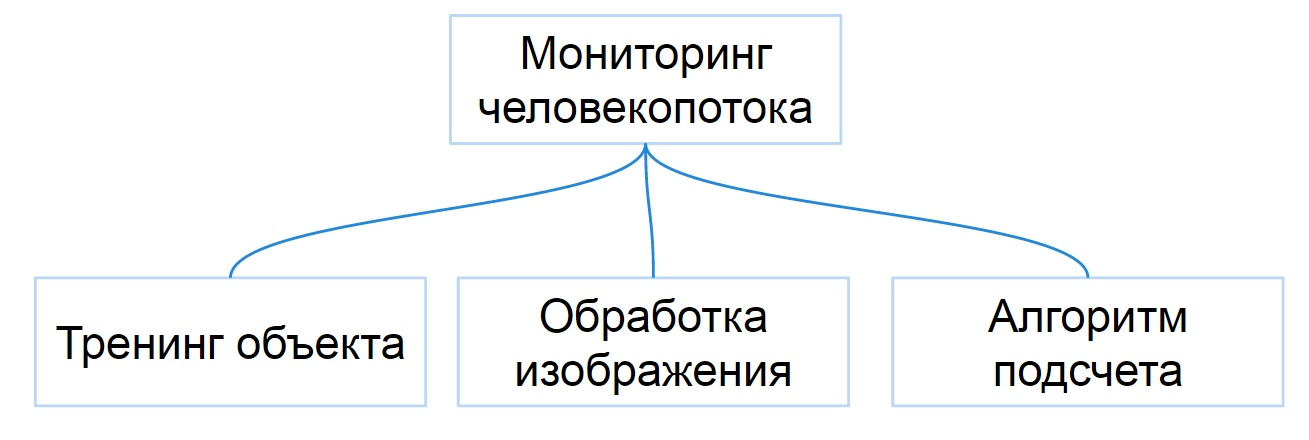
\includegraphics[width=1\textwidth]{pic/conc.jpg}
			\caption{Дерево компонентов системы}
		\end{figure}		

Трекинг объекта задача, которая имеет множество вариантов решений (см. дерево направлений трекинга)

		\begin{figure}[h!]
			\centering
			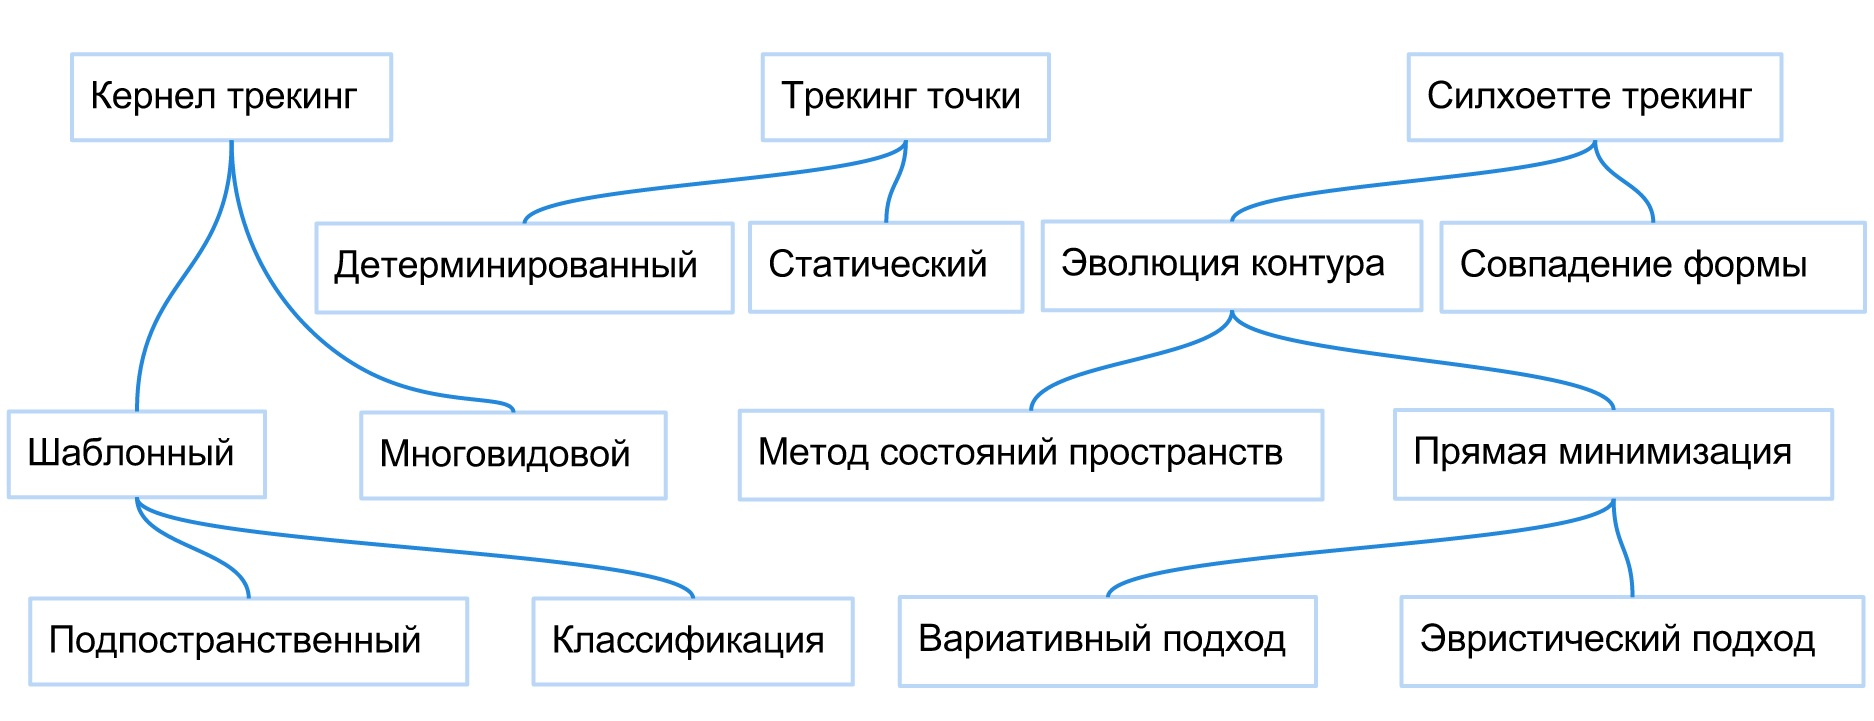
\includegraphics[width=1\textwidth]{pic/tracking_tree.jpg}
			\caption{Дерево направлений трекинга}
		\end{figure}	
Но учитывая используемый алгоритм (вычитание фона), можно получить форму движущегося объекта. Для подсчета нам не важно какой частью тела человек пересекает линию, используемую для подсчета количества людей, поэтому вполне достаточно упростить объект до точки. А из трекинга точки вполне достаточно детерминированного трекинга. 

Для подсчета необходимо разработать алгоритм позволяющий подсчитывать количество треков пересекших в одном или другом направлении линию. 

	\section{Техническое проектирование}
		\subsection{Алгоритм формирования трека}
Задача формирования трека необходима для корректной работы счетчика. 

		\begin{figure}[h!]
			\centering
			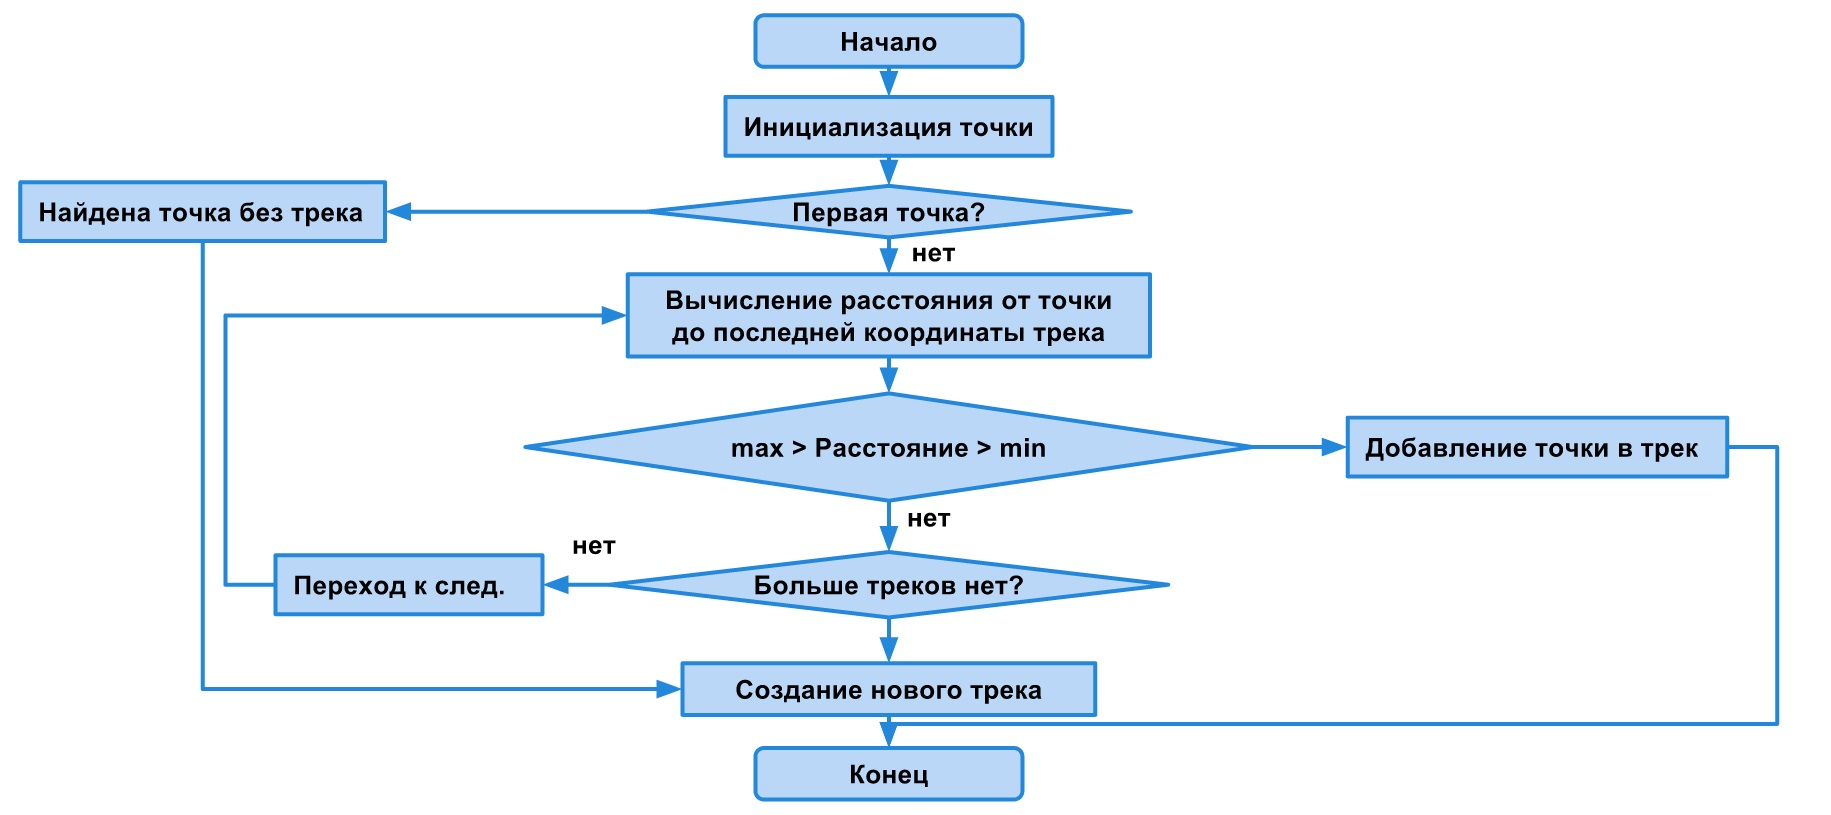
\includegraphics[width=1\textwidth]{pic/new_track_form.jpg}
			\caption{Блок-схема алгоритма формирования трека}
		\end{figure}	

		\subsection{Предотвращение многократного срабатывания}
Для предотвращения некорректного срабатывания счетчика для описания линии используется эпсилон окрестность. В случае если объект будет двигаться вдоль линии это поможет предотвратить многократное срабатывание. Для избавление от многократного срабатывания на одном и том же треке введены условия, что один и тот же трек может однократно идти вниз и вверх. Так как на видео мы видим ограниченную область и люды выходят за пределы этой области, то у трека вводится понятие жизненного цикла. 
		\subsection{Алгоритм работы счетчика}
Формирование трека по большей части необходимо для корректной работы счетчика. Имея трек точность работы счетчика существенно возрастает за счет избавления от ложных срабатываний.
		\begin{figure}[h!]
			\centering
			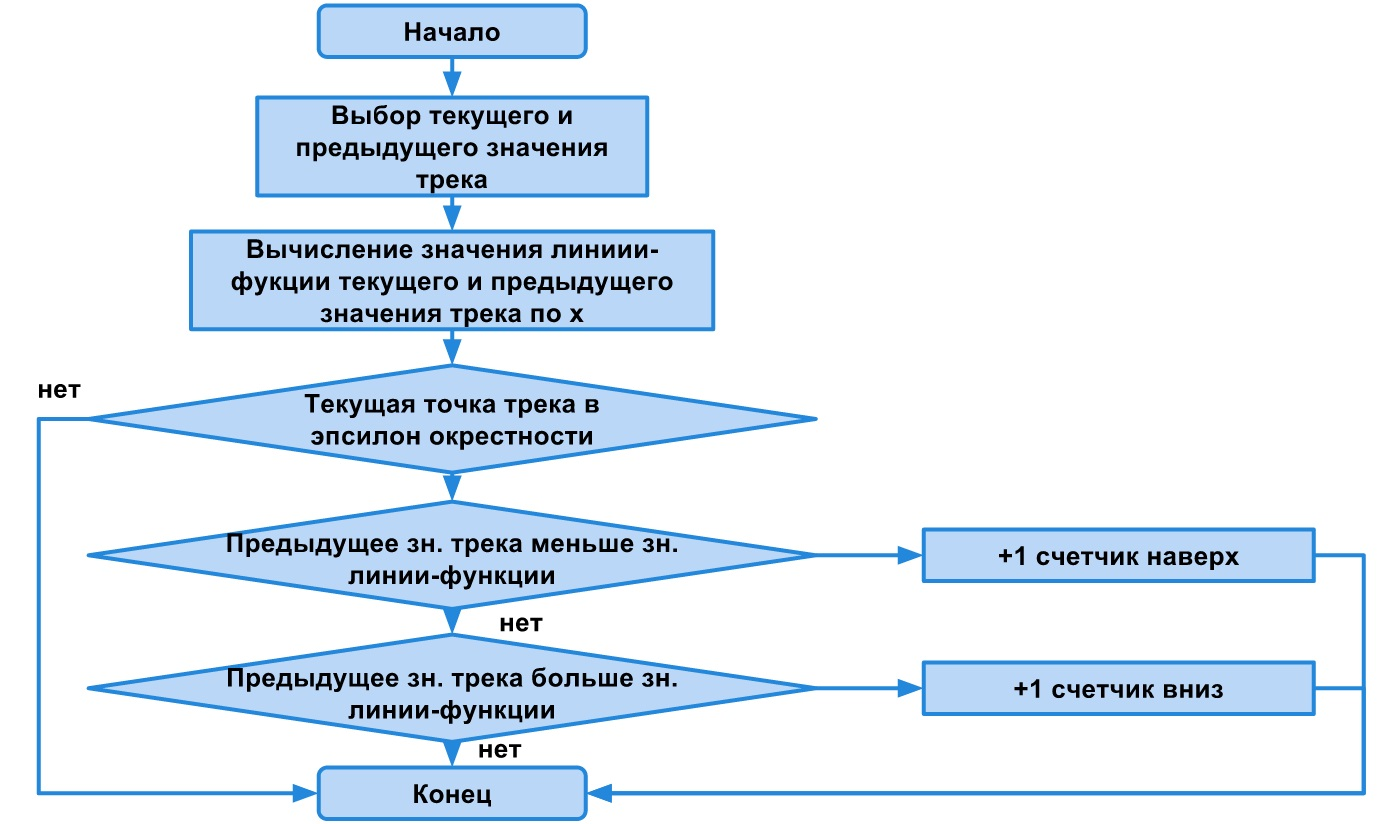
\includegraphics[width=1\textwidth]{pic/counter.jpg}
			\caption{Блок-схема алгоритма работы счетчика}
		\end{figure}	

		\subsection{Описание алгоритма вычитания фона}
Алгоритмы вычитания фона широко применяются в задачах видеонаблюдения и активно изучаются в последнее время. Большинство существующих алгоритмов вычитания фона основываются на сравнении цвета пикселей или блоков очередных кадров со своими цветовыми моделями. При этом значительные перепады в освещении обычно приводят к большому числу ошибок, а иногда и к полной деградации работы системы. В методе, предлагаемом в данной работе, весь кадр видео разбивается на блоки, для каждого из которых на основе бустинга строится отдельный классификатор, определяющий перекрыт данный блок или нет. Благодаря использованию признаков, основанных на сравнении цветов разных пикселей в блоке, достигается большая устойчивость к изменениям освещенности и дрожанию камеры. 

\begin{itemize}
	\item Попиксельные 
	\item Поблочные
	\item Алгоритмы, основанные на Марковских или Условных случайных полях
\end{itemize}


Требуя значительного времени при обучении под новую сцену, на этапе выполнения алгоритм демонстрирует высокую скорость, сравнимую со скоростью простейших алгоритмов вычитания фона. Было проведено сравнение точности сегментации видео с помощью данного алгоритма и нескольких существующих аналогов на выложенных в открытый доступ видеороликах. Сравнение показало высокую точность работы предложенного алгоритма.

Большинство методов вычитания фона можно разбить на 3
категории:



Методы первой категории обрабатывают все пиксели очередного кадра независимо. Цвет каждого пикселя на текущем кадре сравнивается с его цветовой моделью. Типичными цветовыми моделями являются нормальное распределение [1], смесь нормальных распределений [1] и непараметрические модели [2]. Метод [1] предполагает, что значение цвета пикселя фона – случайная величина, чье распределение можно аппроксимировать смесью нормальных распределений. Среди недостатков данного метода можно выделить необходимость использования большого числа гауссиан в смеси для моделирования фона, что приводит к существенным вычислительным затратам. Кроме того,  данный метод чувствителен к небольшим дрожаниям камеры. Методы второй категории независимо обрабатывают не пиксели, а целые блоки. То есть весь кадр разбивается на блоки, и для каждого из них принимается независимое решение. Несмотря на то, что потенциально такие методы не могут быть идеально точными, зачастую они дают более приемлемый результат, т.к. используют для принятия решения информацию с целой области. В эту категорию входят, например, метод на основе построения LBP- гистограмм [10] и метод на основе метрики SSD. Последний метод хранит модель фона в виде одного изображения. Результат на каждом кадре производится с помощью сравнения значения метрики близости с порогом. Метрика считается поблочно и равна сумме квадратов разностей между цветами соответствующих пикселей фона и текущего кадра. Предложенный метод также попадает в эту категорию. В последнее время были предложены методы вычитания фона, проводящие сегментацию пикселей изображения, используя модели Марковского и Условного случайного поля для учета пространственных зависимостей между пикселями [4-5]. С помощью данных методов можно дополнительно требовать, чтобы границы областей объектов переднего плана проходили преимущественно по краям на входном изображении. Но, к сожалению, методы данной категории являются более медленными, и почти не используются на практике в системах видеонаблюдения. 
В работе [3] авторы предлагают алгоритм вычитания фона для использования в видеоконференциях. Поэтому, они используют несколько иную постановку задачи: в качестве переднего плана выступает лишь человек, ближайший к видеокамере. Люди на заднем плане, считаются частью фона. Для решения данной задачи предлагается использовать информацию о наиболее вероятном движении объектов переднего плана. С помощью данного метода можно уменьшить ошибки сегментации из-за движений в фоновом изображении, но с другой стороны необходимо заранее знать наиболее вероятные модели движения для объектов переднего плана, что возможно не в каждом случае. Все алгоритмы вычитания фона условно можно разделить на быстрые, но слабоустойчивые к изменениям освещения и дрожаниям камеры, и качественные, но требующие существенных временных затрат на обработку каждого кадра. Мы предлагаем метод, который может одновременно быстро и качественно решать задачу, основываясь на классификаторах, натренированных для каждого блока. информативные признаки для каждого блока кадра удается выявлять с помощью алгоритма машинного обучения. Для тренировки алгоритма машинного обучения необходима выборка положительных и отрицательных примеров. В общем случае для ее создания необходимо много данных, размеченных вручную. Эта процедура требует больших временных затрат и не гарантирует получение репрезентативной выборки. Поэтому мы генерируем выборку без объектов переднего плана, имитируя возможные изменения в освещении и настройках видеокамеры, а также выборку, имитирующую возможные перекрытия фона. Для
такой генерации достаточно всего одного кадра сцены без объектов переднего плана.  

		\begin{figure}[h!]
			\centering
			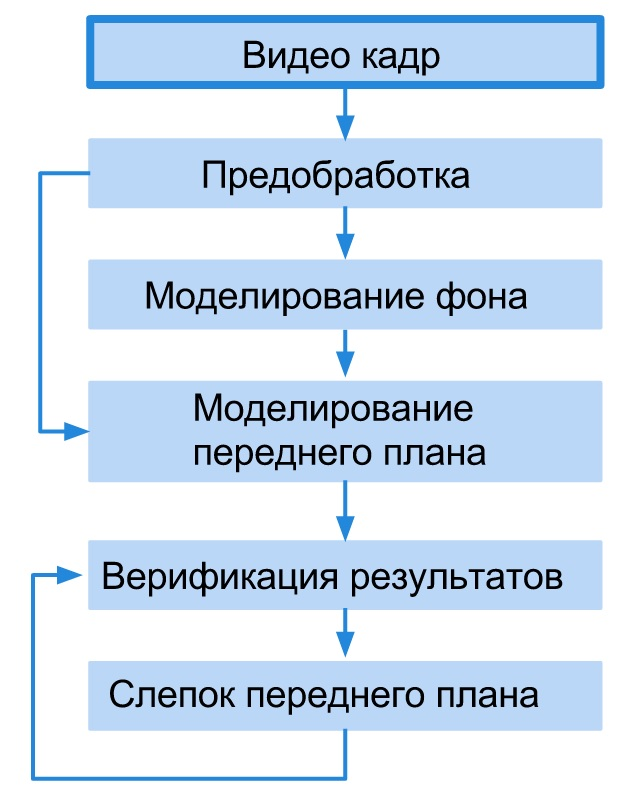
\includegraphics[width=0.5\textwidth]{pic/back_ground_substraction.jpg}
			\caption{Блок-схема алгоритма вычитания фона}
		\end{figure}
	\section{Рабочий этап проектирования системы}	

		\subsection{Визуализация}
Во время анализа видео выполняя любые операции связанные с анализом необходимо визуализировать все изменения. Так имея на входе обычное RGB необходимо преобразовать с кажем в серый. Для того чтобы удостоверится в адекватности проделанных манипуляций нужно вузуализировать каждое действие. Куда более это критично для трекинга. Проверять правильность формирования трека невозможно или чрезвычайно сложно без визуализации. 

		\begin{figure}[h!]
			\centering
			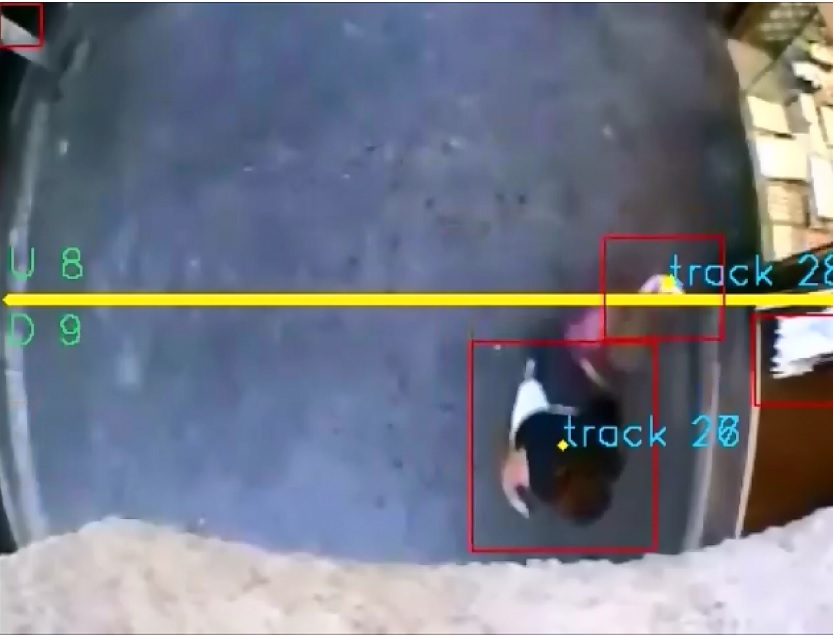
\includegraphics[width=0.5\textwidth]{pic/result_1_1.jpg}
			\caption{Пример обработанного видео}
		\end{figure}	

А наибольший интерес для нас представляет визуализация подсчета людей, а так же детекция их движения. Так движущиеся объекты описываются красными прямоугольниками, а счетчик выполнен в виде цифр над и под пересекаемой линией.

		\subsection{Тестирование}

Тестирования выявило слабые стороны применения данного метода и наиболее частые из них приведены в диаграмме ложных срабатываний
		\begin{figure}[h!]
			\centering
			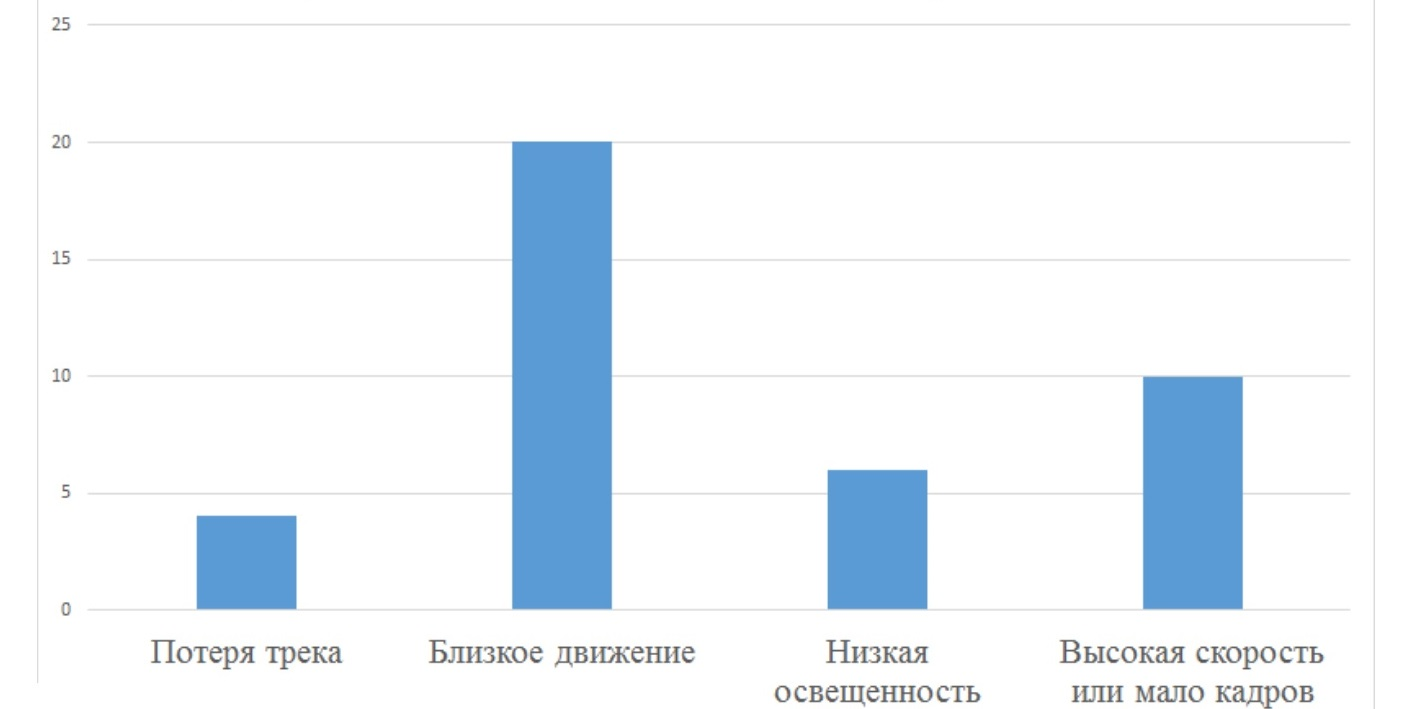
\includegraphics[width=0.5\textwidth]{pic/diogr.jpg}
			\caption{Диаграмма ложных срабатываний}
		\end{figure}

		\subsection{Результаты}
В результате работы мы получили систему позволяющая подсчитывать людей при помощи анализа видео. Общие характеристики данной системы приведены ниже(На основе отладочного видео):
\begin{itemize}
	\item Максимальная точность - 84,5%
	\item Реальное кол-во людей: 32
	\item Подсчитанное кол-во людей: 27
	\item Длительность видео: 75 сек.
\end{itemize}

Система применима для слабопоточных систем с хорошим освещением. К недостаткам следует отнести: некорректное срабатывание при близком движение объектов, необходимость предварительной настройки, работает на любых движущихся объектах и требуется хорошая освещенность. 

		\begin{figure}[h!]
			\centering
			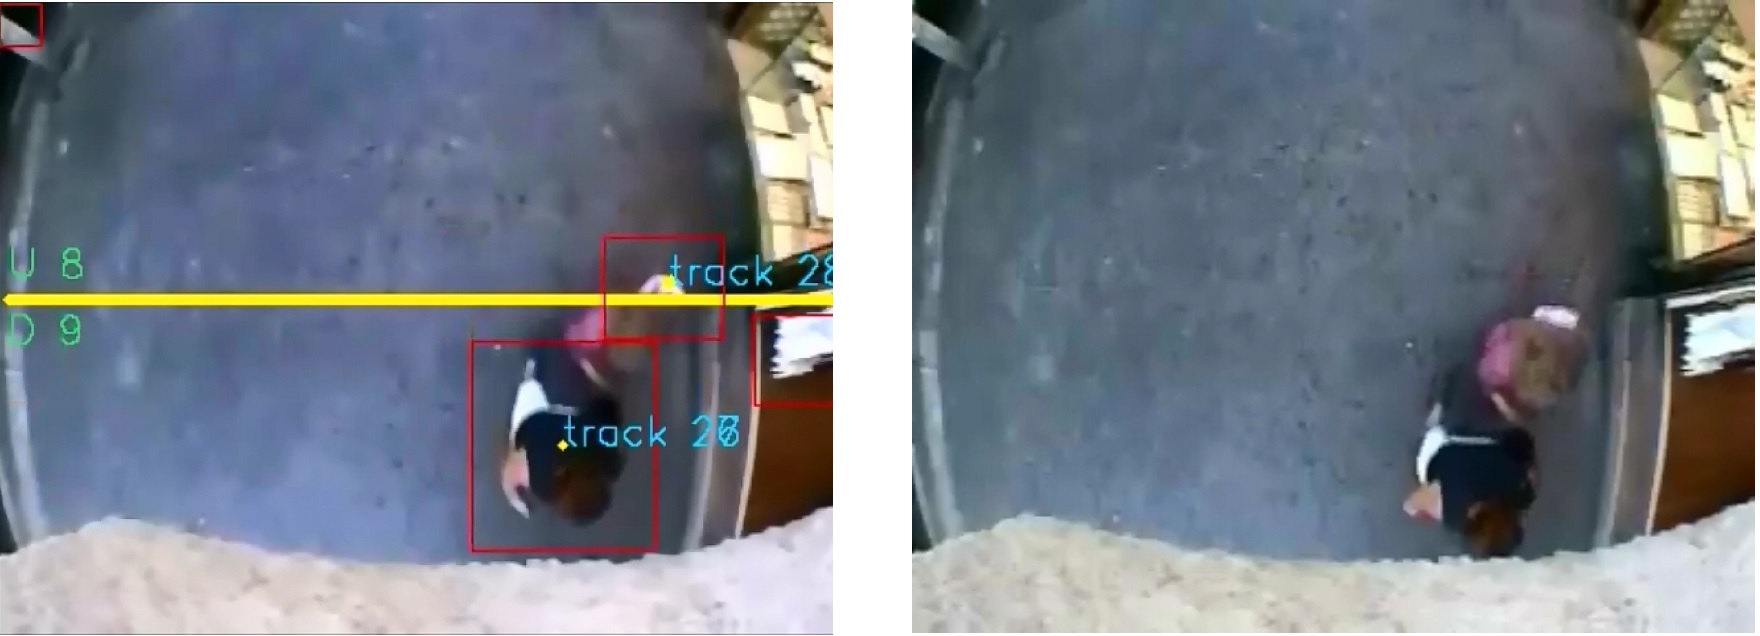
\includegraphics[width=0.9\textwidth]{pic/result.jpg}
			\caption{Результаты работы}
		\end{figure}


\newpage
\subsection{Выводы}

Характеристики:
\begin{itemize}
	\item Система имеет высокую точность*
	\item Быстрая и простая развертка
	\item Применима для любых движущихся объектах
	\item Не требовательна к качеству входного видео
	\item Не подходит для задач с точностью \~ 100\%
	\item Не подходит для сильнопоточных систем 
\end{itemize}

Точность системы не максимальна и может быть повышена. Эта характеристика наиболее критична, что я планирую попробовать сделать в рамкам летней практики. Так планируется добавить возможность подсчета близкоидущих людей. 
		
%====================================================================================
	

%====================================================================================
	%Список Литературы	%====================================================================================

\newpage
\addcontentsline{toc}{part}{Список литературы}

	\bibliographystyle{plain}		
	\bibliography{biblio}
\hspace{\parindent} \hspace{\parindent}

1) Chris Stauffer, W.E.L. Grimson, Adaptive background mixture models for real-time tracking, CVPR 1999

2) Ahmed Elgammal, David Harwood, Larry Davis, Nonparametric model for background subtraction, ICCV, 2000

3) Jian Sun, Weiwei Zhang, Xiaoou Tang, Heung-Yeung Shum, Background cut, CVPR, 2006

4) A. Criminisi, G. Cross, A. Blake, V. Kolmogorov, Bilayer segmentation of live video, CVPR, 2006

5) Желтов С.Ю. и др. Обработка и анализ изображений в задачах машинного зрения. — М.: Физматкнига, 2010. — 672 с.

6) А.А. Лукьяница ,А.Г. Шишкин Цифровая обработка видеоизображений. — М.: «Ай-Эс-Эс Пресс», 2009. — 518 с. 

7) Дэвид Форсайт, Жан Понс Компьютерное зрение. Современный подход = Computer Vision: A Modern Approach. — М.: «Вильямс», 2004. — 928 с. 

8) Paul C. Box, Joseph C. Oppenlander (1976), Manual of traffic engineering studies, Institute of Transportation Engineers, p. 17, retrieved December 21, 2010
	\newpage	%====================================================================================	
	%Приложения
	\definecolor{white}{rgb}{1,1,1}
	\lstset{backgroundcolor=\color{white}, basicstyle=\footnotesize, tabsize=4, frame=none}		%====================================================================================
	\part*{Приложение}
	\addcontentsline{toc}{part}{Приложение A. }
		\begin{lstlisting}[language=Python]

	\end{lstlisting}



	%\newpage
%	\part*{Приложение Б.}
%		\addcontentsline{toc}{part}{Приложение Б. }

%\lstset{caption={Подключение к серверу управления базами данных}}
%\lstinputlisting[language=PHP]{scr.js}

	\newpage	
\end{document}
